\documentclass{scrartcl}

\usepackage{amssymb}
\usepackage{amsmath}
\usepackage{tikz}
\usetikzlibrary{calc}	%for centerarc

\def\centerarc[#1](#2)(#3:#4:#5)% Syntax: [draw options] (center) (initial angle:final angle:radius)
{ \draw[#1] ($(#2)+({#5*cos(#3)},{#5*sin(#3)})$) arc (#3:#4:#5); }

%Laing, R.D. (1970). \textit{Knots}. New York: Routledge.

\begin{document}
	
	%\begin{figure}
	%	\centering
	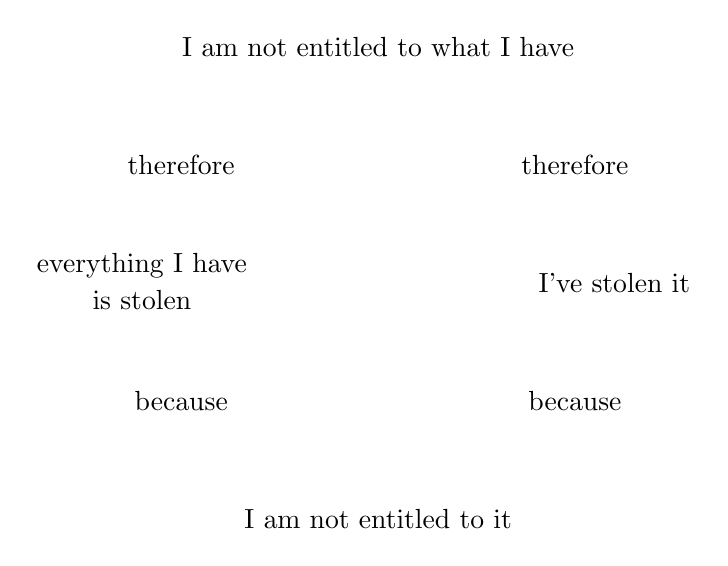
\begin{tikzpicture}
	%\draw[very thick,red] (0,0) circle (3cm);		%for calibrating the arrows
	
	%arrows
	\centerarc[->,>=stealth,very thick](0,0)(35:65:3)	%top left
	\centerarc[->,>=stealth,very thick](0,0)(5:24:3)	%up-mid left
	\centerarc[->,>=stealth,very thick](0,0)(-30:-5:3)	%low-mid left
	\centerarc[->,>=stealth,very thick](0,0)(295:324:3)	%low left
	%
	\centerarc[->,>=stealth,very thick](0,0)(115:144:3)	%top right
	\centerarc[->,>=stealth,very thick](0,0)(156:170:3)	%up-mid right
	\centerarc[->,>=stealth,very thick](0,0)(185:204:3)	%low-mid right
	\centerarc[->,>=stealth,very thick](0,0)(215:245:3)	%low right
	
	\node[fill=white] at (0,3) 		{I am not entitled to what I have};
	\node[fill=white] at (0,-3) 	{I am not entitled to it};
	\node[fill=white] at (-2.5,1.5) {therefore};
	\node[fill=white] at (2.5,1.5) 	{therefore};
	\node[fill=white] at (-3,0.22) 	{everything I have};
	\node[fill=white] at (-3,-0.22) {is stolen};
	\node[fill=white] at (3,0) 		{I've stolen it};
	\node[fill=white] at (-2.5,-1.5){because};
	\node[fill=white] at (2.5,-1.5) {because};
	\end{tikzpicture}
	%	\caption{Laing - \textit{Knots}, p. 35}
	%\end{figure}
	
	
	\vspace{1.5cm}
	
	
	\hspace{1.5cm}		%NB: the hspace is just for centering
	%\begin{figure}
	%	\centering
	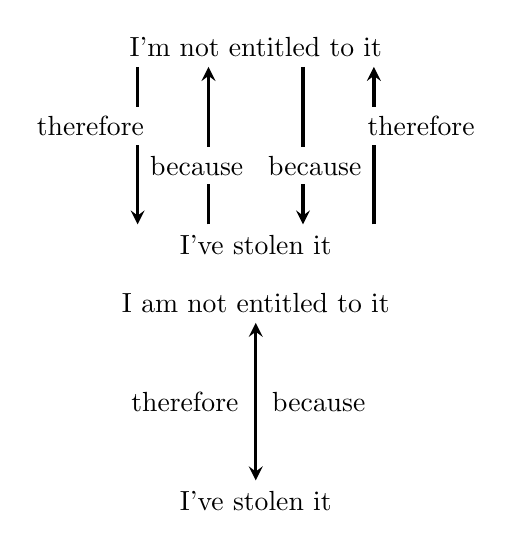
\begin{tikzpicture}
	%top arrows
	\draw[->,>=stealth,very thick]	(-0.6,0.25)--(-0.6,2.25);		%mid-left arrow
	\draw[->,>=stealth,very thick]	(0.6,2.25)--(0.6,0.25);			%mid-right arrow
		\node[fill=white] at (-0.75,1) {because};
		\node[fill=white] at (0.75,1)  {because};
	\draw[->,>=stealth,very thick]	(-1.5,2.25)--(-1.5,0.25);		%leftmost arrow
	\draw[->,>=stealth,very thick]	(1.5,0.25)--(1.5,2.25);			%rightmost arrow
	
	%labels
	\node[fill=white] at (0,2.51)	{I'm not entitled to it};
	\node[fill=white] at (-2.1,1.5) {therefore};
	\node[fill=white] at (2.1,1.5)	{therefore};
	\node[fill=white] at (0,-0.01)	{I've stolen it};
	%NB: the "because" is separate, b/c otherwise the fill overlaps the arrows
	%
	\node[fill=white] at (0,-0.745) {I am not entitled to it};
	\node[fill=white] at (-0.9,-2) 	{therefore};
	\node[fill=white] at (0.8,-2) 	{because};
	\node[fill=white] at (0,-3.255)	{I've stolen it};
		\draw[<->,>=stealth,very thick]	(0,-1)--(0,-3);		%bottom arrow
	\end{tikzpicture}
	%	\caption{Laing - \textit{Knots}, p. 36}
	%\end{figure}
	
	
	\vspace{1.5cm}
	
	
	\hspace{2cm}
	%\begin{figure}
	%	\centering
	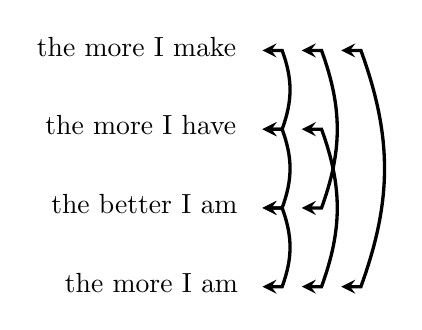
\begin{tikzpicture}[>=stealth]
	%labels
	\node at (0,1.5) 	 {the more I make};
	\node at (0.055,0.5) {the more I have};
	\node at (0.1,-0.5)  {the better I am};
	\node at (0.19,-1.5) {the more I am};
	
	%first layer
	\draw[<->,very thick]	(1.6,1.45)--(1.85,1.45) to[bend left=20] (1.85,0.45)--(1.6,0.45);
	\draw[<->,very thick]	(1.6,0.45)--(1.85,0.45) to[bend left=20] (1.85,-0.55)--(1.6,-0.55);
	\draw[<->,very thick]	(1.6,-.55)--(1.85,-.55) to[bend left=20] (1.85,-1.55)--(1.6,-1.55);
	
	%second layer
	\draw[<->,very thick]	(2.1,1.45)--(2.35,1.45) to[bend left=20] (2.35,-0.55)--(2.1,-0.55);
	\draw[<->,very thick]	(2.1,0.45)--(2.35,0.45) to[bend left=20] (2.35,-1.55)--(2.1,-1.55);
	
	%third layer
	\draw[<->,very thick]	(2.6,1.45)--(2.85,1.45) to[bend left=20] (2.85,-1.55)--(2.6,-1.55);
	\end{tikzpicture}
	%	\caption{Laing - \textit{Knots}, p. 39}
	%\end{figure}
	
	
	\newpage
	
	
	%\begin{figure}
	%	\centering
	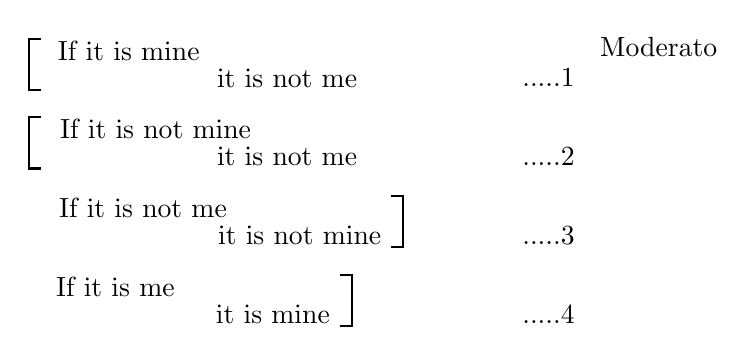
\begin{tikzpicture}
	%labels
	\node at (0.17,3) 		{If it is mine};
	\node at (2.18,2.65) 	{it is not me};
	\node at (0.51,2) 		{If it is not mine};
	\node at (2.18,1.65) 	{it is not me};
	\node at (0.35,1) 		{If it is not me};
	\node at (2.34,0.65) 	{it is not mine};
	\node at (0,0) 			{If it is me};
	\node at (2,-0.35) 		{it is mine};
	
	%numbers
	\node at (6.9,3.05) 	{Moderato};
	\node at (5.5,2.65) 	{.....1};
	\node at (5.5,1.65) 	{.....2};
	\node at (5.5,0.65) 	{.....3};
	\node at (5.5,-0.35) 	{.....4};
	
	%braces
	\draw[thick]	(-0.95,2.5)--(-1.1,2.5)--(-1.1,3.15)--(-0.95,3.15);		%top
	\draw[thick]	(-0.95,1.5)--(-1.1,1.5)--(-1.1,2.15)--(-0.95,2.15);
	\draw[thick]	(3.5,0.5)--(3.65,0.5)--(3.65,1.15)--(3.5,1.15);
	\draw[thick]	(2.85,-0.5)--(3,-0.5)--(3,0.15)--(2.85,0.15);			%bottom
	\end{tikzpicture}
	%	\caption{Laing - \textit{Knots}, p. 41}
	%\end{figure}
	
	
	\vspace{1.5cm}
	
	
	%\begin{figure}
	%	\centering
	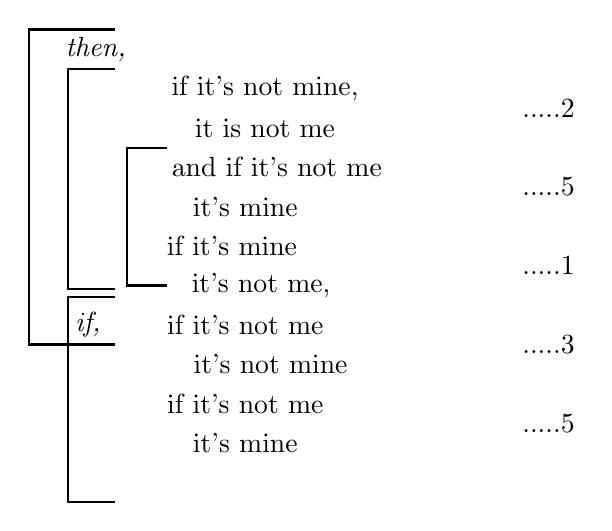
\begin{tikzpicture}
	%labels
	\node at (-1.9,5)  	 {\textit{then,}};
	\node at (0.25,4.5)  {if it's not mine,};
	\node at (0.25,4) 	 {it is not me};
	\node at (0.4,3.5) 	 {and if it's not me};
	\node at (0,3) 		 {it's mine};
	\node at (-0.17,2.5) {if it's mine};
	\node at (0.2,2) 	 {it's not me,};
	\node at (-2,1.5)  	 {\textit{if,}};
	\node at (0,1.5) 	 {if it's not me};
	\node at (0.32,1) 	 {it's not mine};
	\node at (0,0.5) 	 {if it's not me};
	\node at (0,0) 		 {it's mine};
	
	%braces
	\draw[thick]	(-1,2)--(-1.5,2)--(-1.5,3.75)--(-1,3.75);					%innermost
	\draw[thick]	(-1.65,1.95)--(-2.25,1.95)--(-2.25,4.75)--(-1.65,4.75);		%middle top
	\draw[thick]	(-1.65,-0.75)--(-2.25,-0.75)--(-2.25,1.85)--(-1.65,1.85);	%middle bottom
	\draw[thick]	(-1.65,1.25)--(-2.75,1.25)--(-2.75,5.25)--(-1.65,5.25);		%outermost
	
	%numbers
	\node at (3.85,4.25) 	{.....2};
	\node at (3.85,3.25) 	{.....5};
	\node at (3.85,2.25) 	{.....1};
	\node at (3.85,1.25) 	{.....3};
	\node at (3.85,0.25) 	{.....5};
	\end{tikzpicture}
	%	\caption{Laing - \textit{Knots}, p. 43}
	%\end{figure}
	
	
	\vspace{1.5cm}
	
	
	\hspace{-1.25cm}
	%\begin{figure}
	%	\centering
	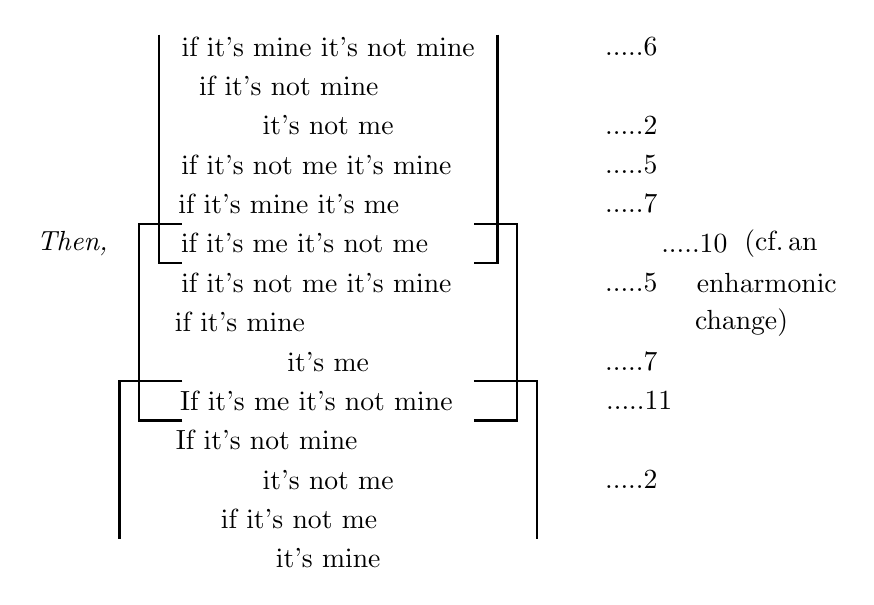
\begin{tikzpicture}
	%labels
	\node at (0,6.5) 	{if it's mine it's not mine};
	\node at (-0.5,6) 	{if it's not mine};
	\node at (0,5.5) 	{it's not me};
	\node at (-0.15,5) 	{if it's not me it's mine};
	\node at (-0.5,4.5) {if it's mine it's me};
	\node at (-3.25,4) 	{\textit{Then,}};
	\node at (-0.3,4) 	{if it's me it's not me};
	\node at (-.15,3.5) {if it's not me it's mine};
	\node at (-1.12,3) 	{if it's mine};
	\node at (0,2.5) 	{it's me};
	\node at (-0.15,2) 	{If it's me it's not mine};
	\node at (-.78,1.5) {If it's not mine};
	\node at (0,1) 		{it's not me};
	\node at (-.37,0.5) {if it's not me};
	\node at (0,0) 		{it's mine};
	
	%braces
	\draw[thick]	(-2.15,6.65)--(-2.15,3.75)--(-1.85,3.75);
	\draw[thick]	(2.15,6.65)--(2.15,3.75)--(1.85,3.75);
	\draw[thick]	(-1.85,1.75)--(-2.4,1.75)--(-2.4,4.25)--(-1.85,4.25);
	\draw[thick]	(1.85,1.75)--(2.4,1.75)--(2.4,4.25)--(1.85,4.25);
	\draw[thick]	(-1.85,2.25)--(-2.65,2.25)--(-2.65,0.25);
	\draw[thick]	(1.85,2.25)--(2.65,2.25)--(2.65,0.25);
	
	%numbers
	\node at (3.85,6.5) 	{.....6};
	\node at (3.85,5.5) 	{.....2};
	\node at (3.85,5) 		{.....5};
	\node at (3.85,4.5) 	{.....7};
	\node at (4.65,4) 		{.....10};
		\node at (5.75,4) 	{(cf.$\,$an};
		\node at (5.57,3.5) {enharmonic};
		\node at (5.25,3) 	{change)};
	\node at (3.85,3.5) 	{.....5};
	\node at (3.85,2.5) 	{.....7};
	\node at (3.95,2) 		{.....11};
	\node at (3.85,1) 		{.....2};
	
	\end{tikzpicture}
	%	\caption{Laing - \textit{Knots}, p. 45}
	%\end{figure}
	
\end{document}